\chapter{序論}
\thispagestyle{empty}
\label{chap1}
\graphicspath{{chap1/figure/}}
\minitoc

%%%%%%%%%%%%%%%%%%%%%%%%%%%%%%%%%%%%%%%%%%%%%%%%%%%%%%%%%%%%%%%%%%%%%%%%%%%%

% ================================================== %
% section
% ================================================== %
\newpage
\section{研究の意義・背景}
\label{chap1_background}

通常、我々が天体を観測するとき、可視光を通してその形状や特徴を観察する。
一方で、天文学においては熱や電磁波、放射線といった可視光以外の媒体を通じて様々な現象が明らかにされてきた。
中でも、電磁波の一種であるX線を観測することは、天文学において非常に有用な価値を持つ。
2018年に打ち上げられたFOXSI3では太陽コロナのX線写真を撮影することに成功し、その物理をより明らかにするに至った。\cite{weko_20796_1}
図\ref{fig:foxsi-fullsun-image}はその撮影像の1枚である。
太陽コロナを満たす高温のプラズマから放射される電磁波はX線の領域にあたり、これを撮影することは長年の課題であった。
X線は大気により吸収されやすいという特徴を持ち、地上での観察が困難であるため、大気圏外に打ち上げられた宇宙船上での撮影が求められるからである。
X線に対して集光効率がよく、天体分野において広く応用されるミラー結像系だが、運動中のロケットから対象物を撮影する際に生じる角度誤差に対するロバスト性の低さが難点になっている。
この問題に対する一つの解決策として与えられたのが、Wolterらが提案した2回反射により角度誤差耐性を強めたWolter型ミラーである。\cite{1952AnP...445...94W}
Wolter型のミラーを導入していたFOXSI3では、無事その撮影に成功し、十分実用的な光学系であることが実証された。
より高分解能な太陽コロナの像を撮影することを目標として、2023年頃光学系をアップデートしたFOXSI4が打ち上げを予定しているが、ここでもまたWolter型ミラーが搭載される。\cite{2019AGUFMSH31C3315V}
Wolterミラーの加工精度を向上させ、結像性能を高めることは、得られる像の質を上げることに繋がる。

\begin{figure}[h]
\centering
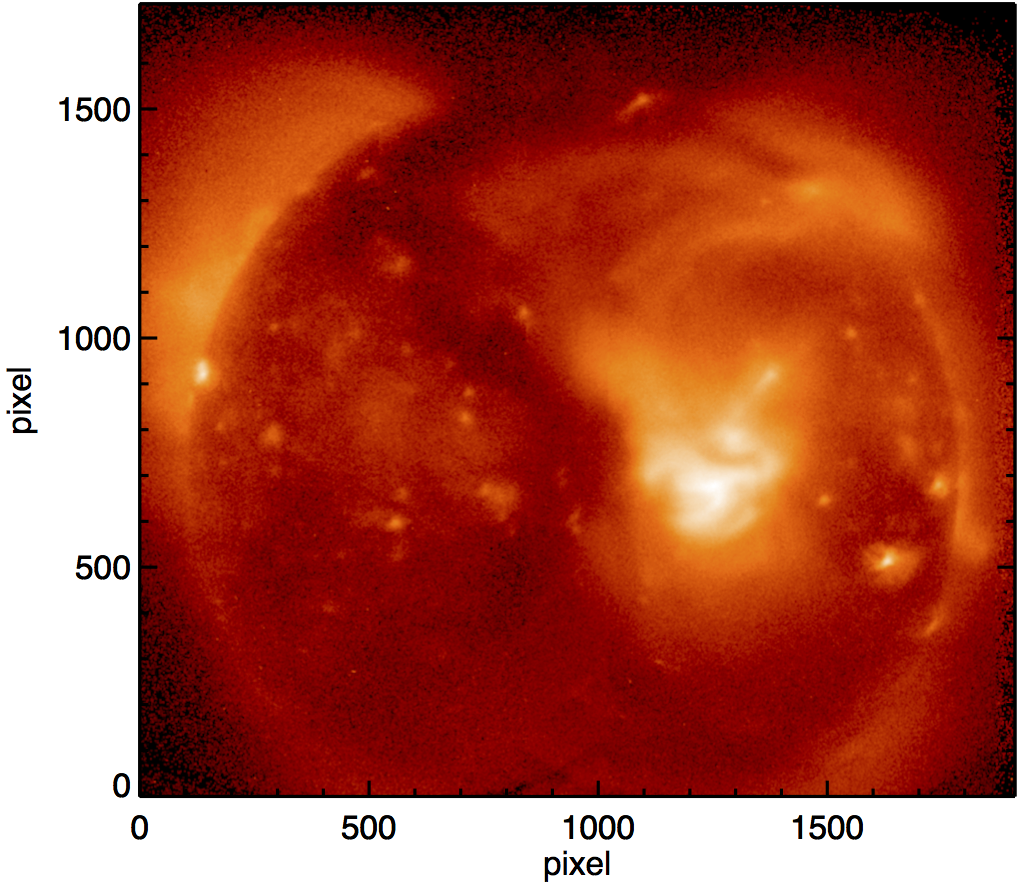
\includegraphics[width=6cm]{foxsi3-full-sun.png}
\caption{FOXSI-3 phoenix full sun soft X-ray image}
\label{fig:foxsi-fullsun-image}
\end{figure}

\clearpage
% -------------------------------------------------- %
% section
% -------------------------------------------------- %
\newpage

\section{Wolterミラー}
\label{chap1_wolter_mirror}

\begin{figure}[b]
\centering
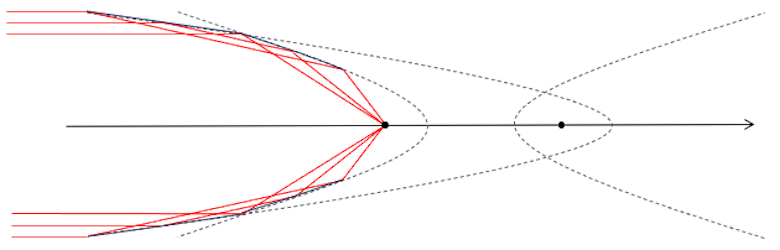
\includegraphics[width=10cm]{wolter_type_1.png}
\caption{Wolter I型}
\label{fig:wolter_type_1}
\end{figure}

\begin{figure}[b]
\centering
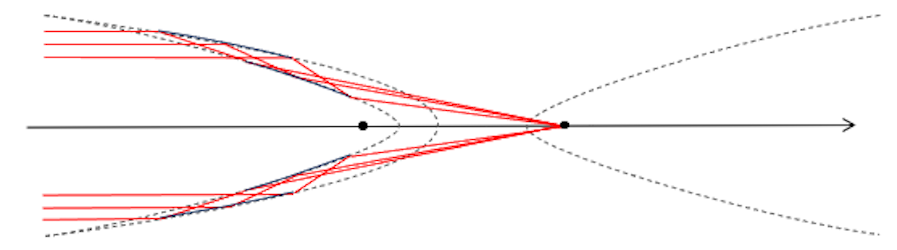
\includegraphics[width=10cm]{wolter_type_2.png}
\caption{Wolter II型}
\label{fig:wolter_type_2}
\end{figure}

\begin{figure}[b]
\centering
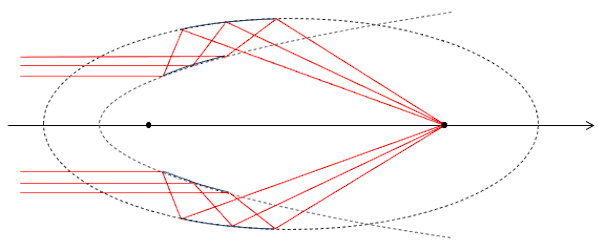
\includegraphics[width=10cm]{wolter_type_3.png}
\caption{Wolter III型}
\label{fig:wolter_type_3}
\end{figure}

光を集光・結像するための素子として、反射を利用するミラー、回折を利用するフレネルゾーンプレート、屈折を利用するレンズなどが広く使用されている。
より高強度の像が求められる天体観測の分野では、基本的にミラーによる結像系が採用される。
フレネルゾーンプレートは遮蔽・透過の領域を環状に並べていく光学素子であることから、原理上効率が高くないことが知られている。
また、口径を大きくできないという問題があり、これもまた天体観測に適さない大きな要因となっている。
レンズは波長の短いX線の領域では集光効率が悪化する。
波長の短い領域の電磁波に対して、物質の屈折率はほとんど1に近い値を取るため、屈折による変化は僅かなものとなる。
そのため、十分な屈折率を確保するためにレンズを重ねていくと、多数のレンズにより吸収され、集光効率が悪化してしまうのである。
以上のことから、天体の分野、とりわけX線の領域での観察においては、ミラー結像系が用いられる。

十分遠方にある天体を観測する際、それが発するまたは反射する光はほぼ平行光とみなせる。
放物線の持つ平行線を反射して焦点に集めるという効果を利用して、放物線を軸回りに回転した曲面で平行光を反射し1点に集める光学素子が回転放物面ミラーである。
全周に渡って回転した回転放物面ミラー(図\ref{fig:parabola_rotation_mirror})は、円形に広がる平行光に対してこれを1点に集光する。

\begin{figure}[b]
\centering
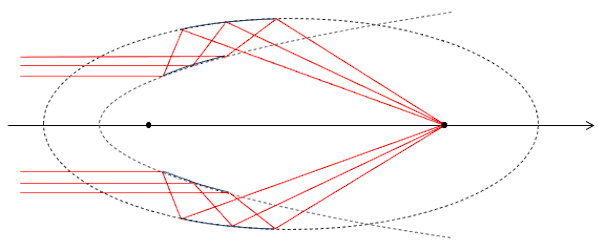
\includegraphics[width=10cm]{wolter_type_3.png}
\caption{回転放物面ミラー}
\label{fig:parabola_rotation_mirror}
\end{figure}

しかし、回転放物面には設置角度の誤差に弱いという欠点が存在する。
これを解決するのが、2回反射型のミラーである。
図\ref{fig:canceling_angle_error_by_two_reflections}に示すように、一般に同じ角度誤差が生じるような2枚のミラーで1回ずつ反射をすると最終的に出射される光は設置角度誤差の影響を受けない。

\begin{figure}[b]
\centering
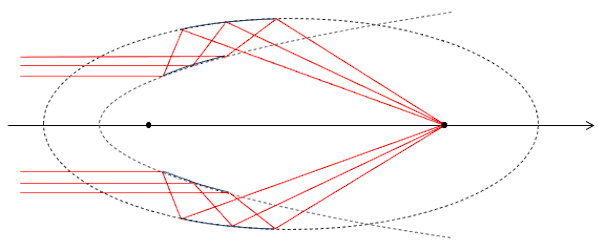
\includegraphics[width=10cm]{wolter_type_3.png}
\caption{2回反射による設置角度誤差のキャンセル}
\label{fig:canceling_angle_error_by_two_reflections}
\end{figure}

これは、2回反射が設置角度誤差への耐性において有利であることを示す。
また、1回反射の放物面ミラーは、アッベの正弦条件を満たさない。
ただし、無限遠の光源に対するアッベの正弦条件は図\ref{fig:abbe_sine_condition_for_parallel_light}の変数について
\[
    x = f \sin u
\]
と表される。

\begin{figure}[b]
\centering
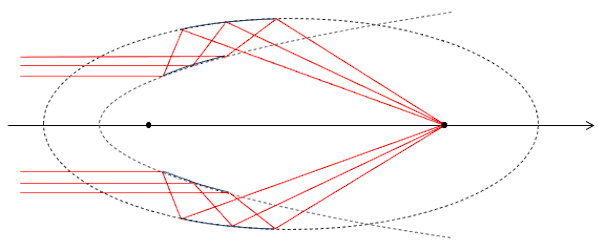
\includegraphics[width=10cm]{wolter_type_3.png}
\caption{無限遠の光源に対するアッベの正弦条件}
\label{fig:abbe_sine_condition_for_parallel_light}
\end{figure}

アッベの正弦条件を満たすとき、光軸上の結像に球面収差およびコマ収差が乗らない系となる。
2回反射を利用した集光ミラーであって、全周にわたって回転したものをWolterミラーという。
2回の反射面は、放物線、双曲線、楕円の3種類の2次曲線を組み合わせた図形の回転体として与えられる。
焦点を共有するように設計・配置することで1点に集光する系を構成することができる。
その他にも、板型の部分回転面を2つ用いるものや、同じく板型で4回に分けて反射するKBミラーが存在する。
口径を大きくでき、また受光面積の面で有利であるため、天体の分野では全周に渡る回転体であるWolterミラーが採用されている。
WolterミラーにはI型(図\ref{fig:wolter_type_1})、II型(図\ref{fig:wolter_type_2})、III型(図\ref{fig:wolter_type_3})の3種類が存在する。
I型は放物面、双曲面の順に反射する。
いずれも内面で反射する形状になっているため、\ref{chap1_wolter_fabrication_process}節で述べるマンドレル転写加工がしやすく高精度な作製が期待できる。
また、受光面積を広げるため、\ref{chap1_nested_wolter_mirror}節で述べるような複数枚のネスト構造を構成することが比較的容易である。
II型は放物面内面、双曲面外面の順に反射する構成になっている。
I型に比べ加工・設置が難しくなるが、2枚が覆いかぶさるように重ねた配置にすることができ、焦点距離を短くし光学系全体を小型化することができる。
III型も同様に加工・設置が難しくなるが、焦点距離を短くするような配置が可能になる。
II型、III型は凸面形状ミラーの加工の困難さからWolterミラーとしては実用化されていない。
KB型配置ではIII型に対応する構成での集光光学系が提案されている。\cite{Yamada:20}

\subsection{ネスト型Wolterミラー}
\label{chap1_nested_wolter_mirror}

Wolterミラーのような円筒形のミラー、特にX線を反射するため斜入射角が小さく設計されたミラーにおいて、中空になっている内側部分を通過する光を集めることができず、主に遮蔽して捨てることになる。
これは、集光強度を高める上で不利な構成になってしまう。
これを解決する方法として、図\ref{fig:nested_wolter_mirror}のように口径の異なるWolterミラーを内側に挿入するというものある。

\begin{figure}[b]
\centering
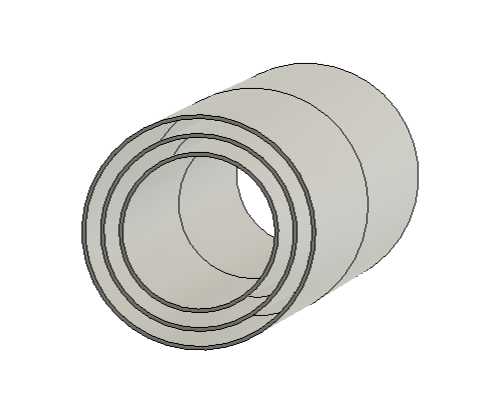
\includegraphics[width=8cm]{nested_wolter_mirror.png}
\caption{Nested Wolterミラーの例}
\label{fig:nested_wolter_mirror}
\end{figure}

このようにネスト構造にすることで、受光面積を大きくすることができ、集光強度を上げることができる。
このようなネスト構造を構成できるのはI型のみであり、その点で天体応用としてはI型が有力な選択肢となる。
実際、FOXSI3でもI型をネストしたNested Wolterミラーが搭載されていた。
このように受光面積の観点では非常に有利であるNested Wolterミラーだが、ネストする枚数を増やすほどその設置が困難になるという問題がある。
ミラー同士の角度・光軸のずれなど、調整しなければならない誤差要因が増えるためである。
そのため、ネストの構成後に光学系を統合的に計測する方法が必要になる。
また、ミラー同士をネストさせたあとにプローブを挿入して計測することは困難であるため、その統合的な評価は間接測定によって行われなければならない。

\clearpage
% -------------------------------------------------- %
% section
% -------------------------------------------------- %
\newpage
\section{天文用大型Wolterミラーの製造プロセス}
\label{chap1_wolter_fabrication_process}

ここで、測定対象となるWolterミラーの製造プロセスについて述べる。

凸形状のマンドレルを作製する
電鋳加工する
などなど

\subsection{直接計測法}


久米らは、周方向形状誤差プロファイルおよび長手方向形状誤差プロファイルを数本ずつ取得し、これらを組み合わせることで3次元形状を決定するという方法を提案した。\cite{Kume2017}
しかし、これらのプロファイル計測がある始点からの変位量を測定するという手法を取る以上、それぞれ直径と長手プロファイルの傾き(テーパー角)の情報を取得することができない。
このようなプロファイル計測では得られない情報を取得する計測方法が必要である。

\clearpage
% -------------------------------------------------- %
% section
% -------------------------------------------------- %
\newpage
\section{波面計測法によるミラー形状の解析}
\label{chap1_method_for_mirror_metric}

プロファイル計測では得られない情報を取得すること、またネスト構造のミラーを計測可能な間接測定であることという2つの要請を満足させる方法として、波面計測法がある。
波面計測法は波動光学に基づく計測法であり、また本研究ではとりわけスカラー回折理論に基づいた波面計測法について扱う。
光の波動場は振幅と位相を持つ複素スカラー場として与えられ、単色光に関してはこれを複素スカラー場として重ね合わせることで干渉を表現する。
図hogeに示すように、ミラー形状に誤差が乗っているとき、その集光波面は理想的な球面波ではなく誤差に応じた変化が見られる。
このことを利用し、集光波面の位相分布の理想状態との変量を解析することで形状誤差分布を求めるというのが波面計測法の基本的な方針となる。
波面計測法の基盤となる集光波面の複素波動場を計測・算出する方法として、様々な方法が知られている。


\clearpage
% -------------------------------------------------- %
% section
% -------------------------------------------------- %
\newpage

\section{本研究で測定対象となるWolterミラー}
\label{chap1_target_wolter}

\subsection{設計}
\label{chap1_wolter_arrangement}
本研究において測定対象となるのは、FOXSI-4での利用が検討されている天体望遠鏡用のWolterミラーであり、放物面、双曲面の順に反射するI型に分類される。
現在、回転体ミラーの加工では凸形状のマンドレルを高精度に加工し、そこに金属材料を転写するという方式が非常に有利であり、反射面がいずれも内側になるWolter I型が採用されている。
また、放物面と双曲面が連続に接続されている方が端面が存在しないぶん加工精度の点で有利であるため、そのような構成となっている。

以下では、開発対象となっているWolter I型のミラーの設計パラメータを図\ref{fig:wolter_params}に対応して表\ref{tb:wolter_params}に示す。

\begin{figure}[h!]
\centering
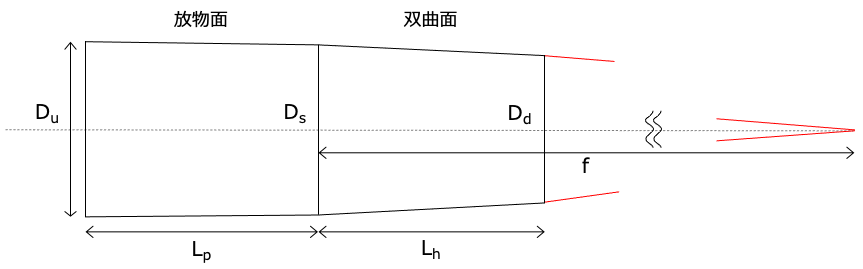
\includegraphics[width=12cm]{wolter_mirror_params.png}
\caption{Wolterミラーの設計変数}
\label{fig:wolter_params}
\end{figure}

\begin{table}[ht]
\begin{center}
  \begin{tabular}{|c|c|l|} \hline
    変数 & 値 & 説明 \\ \hline
    $d_u$ & 60.801 mm & 上流端開口直径 \\
    $d_s$ & 60.000 mm & 接合部直径 \\
    $d_d$ & 57.689 mm & 下流端開口直径 \\
    $l_p$ & 102.501 mm & 放物面部長さ \\
    $l_h$ & 97.499 mm & 双曲面部長さ \\
    $ml$ & 200.000 mm & ミラー全長 \\
    $f$ & 2000.000 mm & 焦点距離 \\ \hline
  \end{tabular}
  \caption{Wolterミラー各設計変数の値}
  \label{tb:wolter_params}
\end{center}
\end{table}

これらを図\ref{fig:wolter_profile}のように放物面部および双曲面部の設計半径として表すと、下式(パラメータは図\ref{tb:wolter_profile_constants})のようになる。
$f1$は座標系の平行移動に関して任意であるため、変数として表記する。

\begin{equation}
    r_p(z) = \sqrt{ -4p(z - p - f_2) } \\
\end{equation}

\begin{equation}
    r_h(z) = b \sqrt{ \frac{(z - (f_1 + f2) / 2)^2}{a^2} - 1.0 }
\end{equation}

\begin{figure}[h]
\centering
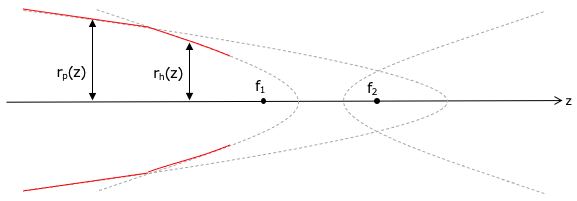
\includegraphics[width=10cm]{mirror_profile.png}
\caption{Wolterミラーの設計半径}
\label{fig:wolter_profile}
\end{figure}

\begin{table}[htb]
    \begin{center}
      \begin{tabular}{|c|c|l|} \hline
        定数 & 値 & 説明 \\ \hline
        $p$ & 0.0562 mm & 下流端開口直径 \\
        $a$ & 1000.056 mm & 放物面部長さ \\
        $b$ & 10.606 mm & 双曲面部長さ \\ 
        $f_1$ & 任意 & 焦点座標 \\
        $f_2$ & $f_1 + \sqrt{ a^2 + b^2 }$  & 共焦点座標 (双曲線のもう一方の焦点) \\\hline
      \end{tabular}
      \caption{Wolterミラーの設計半径における定数}
      \label{tb:wolter_profile_constants}
    \end{center}
\end{table}

\subsection{天文用X線Wolterミラーの持つ特性}
\label{chap1_wolter_specific_feature}

口径が大きく、X線に対応するため射入射角を小さく設定したWolterミラーはNAがやや小さくなり、波面計測において求めなければならない波面は図\ref{fig:wolter_thinring}に示すように非常に細い輪帯状になる。
輪帯の幅(外円と内円の半径の差)は実に\SI{363.3}{\micro \metre}であり、波面計測に求められる空間分解能は非常に高いものとなる。
半径方向の位相分布を見る際、極値を取っている状態を判別するには、少なくとも3ピクセルに分割できている必要があり、\SI{100}{\micro \metre}程度の空間分解能で計測できなければならない。
波面精度を十分に確保しつつ、空間分解能が十分に高い波面計測法を開発する必要がある。

\begin{figure}[h!]
\centering
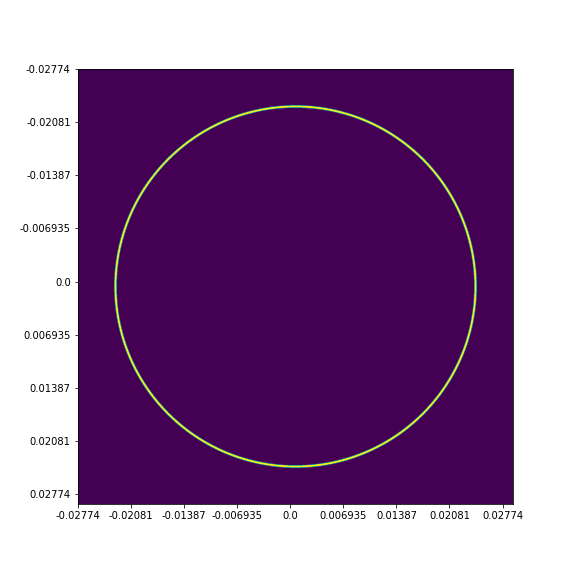
\includegraphics[width=7cm]{wolter_thinring.png}
\caption{Wolterミラー下流端面における集光波面}
\label{fig:wolter_thinring}
\end{figure}


\clearpage
% -------------------------------------------------- %
% section
% -------------------------------------------------- %
\newpage
\section{本論文の目的}
\label{chap1_purpose}

JAXAの進めるミッションLynxでは、0.5秒角分解能の望遠鏡の搭載を大きな目標として掲げている。\cite{Gaskin2019}
これに先立って、2023年に打ち上げられるFOXSI4に搭載するWolterミラーの加工について、1秒角分解能を目標として設定する。
これを実現する上で問題となる加工誤差はどのようなものであるかを統合的な計測から測定し、加工プロセスへ直ちにフィードバックするための系を開発することが、本研究の目的となる。

% -------------------------------------------------- %
% section
% -------------------------------------------------- %
\section{本論文の構成}
\label{chap1_outline}

\ref{chap2}章では、測定対象のWolterミラーに対して様々な種類の誤差を与え、その際の集光波面の変化をシミュレーションする。
この集光波面の強度分布から、目標とする1秒角分解能の達成に際して要求される許容誤差の範囲を見積もるとともに、\ref{chap3}章以降で扱う波面計測法における解析に用いる基底を前もって解析しておく。
\ref{chap3}章では、波面計測における様々な手法の中でWolterミラーの計測に適した方法を検討するため、シミュレーションによってその利点・欠点を洗い出し、最終的に計測に用いる方法を決定する。
\ref{chap4}章では、\ref{chap3}章で提案された手法について、ミラーに比べ加工誤差が小さく、より理想的な集光が期待できるレンズを用いて、その正当性を実証する。
\ref{chap5}章では、実際に加工された3枚の天文用Wolterミラーに対して計測実験を行い、\ref{chap2}でシミュレーションによって求めた誤差応答との比較からミラー内部形状の誤差に関する解析を行う。
最後に、\ref{chap6}章で考察、結論および今後の展望について述べる。

%%%%%%%%%%%%%%%%%%%%%%%%%%%%%%%%%%%%%%%%%%%%%%%%%%%%%%%%%%%%%%%%%%%%%%%%%%%%%
%%% Local Variables:
%%% mode: katex
%%% TeX-master: "../thesis"
%%% End:
